\documentclass[12pt]{article}
\usepackage{amsmath,amsfonts}
\usepackage{graphicx}
\usepackage{enumerate}
\usepackage{algpseudocode}
\usepackage{tikz}
\renewcommand{\thesection}{Problem \arabic{section}}
\renewcommand{\thesubsection}{(\alph{subsection})}
\usepackage{fullpage,url,amssymb,epsfig,color,xspace}

\newcommand{\class}{ECE 358}
\newcommand{\subtitle}{Pencil-n-Paper Assignment 4}

\usepackage[pdftitle={\class \subtitle},%
pdfsubject={University of Waterloo, \class, Spring 2017},%
pdfauthor={Shiranka Miskin}]{hyperref}

%this marks the beginning of the document. Everything before this is called the Preamble.
\begin{document}
\begin{center}
{\Large\bf University of Waterloo}\\
\vspace{3mm}
{\Large\bf \class, Spring 2017}\\
\vspace{2mm}
{\Large\bf \subtitle}\\
\vspace{3mm}
\textbf{Shiranka Miskin, Dhruv Lal, Sam Maier}
\end{center}

\section{}

The only difference between \texttt{rdt 3.0} and \texttt{rdt 2.2} is on the
sender side.  In the following diagram only the "Wait for 0 from below" side of
the FSM is shown, as the other "Wait for 1 from below" state is a near exact
copy, simply with 1 replaced with 0.

\begin{figure}[!htb]
   \center
   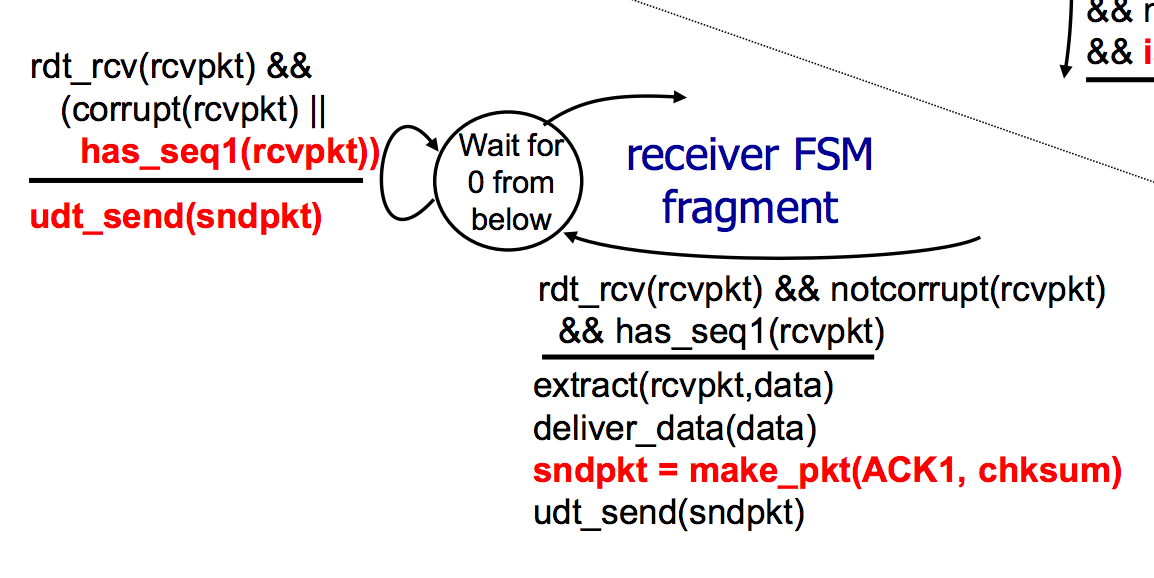
\includegraphics[width=12cm]{fsm-receiver-22.png}
\end{figure}

\section{}

The only case where the receiver will accept a packet is if the sequence number
of the packet matches its expected sequence number.  This means the only way for
a packet to be delivered out of sequence would be if either packet $i + 2^k$ is sent
and received without packet $i$ being received first, or packet $i .. i + 2^k$
are sent and received, but packet $i$ is then resent.

\subsection{}
Since the window size is $\leq 2^k - 1$, packet $i + 2^k$ cannot be sent until
packet $i + 1$ has been acknowledged.  Packet $i + 1$ is only acknowledged once
packet $i$ has been received, therefore the first case is impossible.

Packet $i + 2^k - 1$ is sent only once packet $i$ is acknowledged.
Since packets are never reordered, even if packet $i$ is heavily delayed, that
would mean the following packets are also delayed, therefore the only difference
would be that packet $i$ might be resent and received by the receiver after it
receives some number of packets in $[i, i + 2^k - 2]$.  If the receiver never
received packet $i$, it would ignore all other packets until it gets the packet
$i$ that was resent, and order would still be preserved.  In all other cases,
the receiver's expected sequence number would be $\in [i + 1, i + 2^k - 1]$,
therefore the resent packet $i$ would be ignored.  Only once packet $i + 2^k -
1$ is sent will the expected sequence number be $i$ again, but that packet will
not be sent until packet $i$ has already been successfully acknowledged.  For
these reasons the second case is also impossible, therefore the assertion holds.


\subsection{}
This assertion would not hold in the unlikely case that:
\begin{enumerate}
      \item Packets $i .. i + 2^k - 2$ are sent
      \item The timeout completes, packet $i$ is resent and received by the
receiver
      \item Packets $i + 1 .. i + 2^k - 2$ are received
      \item The sender receives acks for those packets and the resent packet,
         then sends packet $i + 2^k - 1$
      \item The receiver receives packet $i + 2^k - 1$ and sets its expected
         sequence number to $i$
      \item The first packet $i$ that the sender sent is finally received by the
         receiver
\end{enumerate}
Since the receiver was expecting number $i$, it will accept the result and we
will have a duplicated and out of order packet sent to the application.


\section{}
\subsection{}
No incorrectness is introduced as the receiver will always respond with the
sequence number that it expects to receive next.  A duplicate will not change
this value, therefore no incorrectness is introduced.

\subsection{}
It wouldn't introduce any incorrectness, but it may introduce some inefficiency.
Suppose packet $i$ and $i + 1$ are sent, then the ack for packet $i$ is received
right before the timeout, but the ack for packet $i + 1$ is lost.  With minimal
transmission delay, both packets $i$ and $i + 1$ were sent at around the same
time, however since the ack for packet $i$ resets the timer, the effective timer
for packet $i + 1$ is now slightly less than twice the usual timeout.

\subsection{}
The receiver always sends back the value of the next ack it expects to receive,
however on reception of an ACK, the sender sets its base to
\texttt{getacknum(rcvpkt) + 1}.  This sets the base to after the expected
sequence number, which means it will skip that packet when the timeout clears.
A fix would be to have the sender set its base to \texttt{getacknum(rcvpkt)} on
\texttt{rdt\_rcv(rcvpkt) \&\& notcorrupt(rcvpkt)}.

\subsection{}
This would allow for packets to be delivered out of sequence at the receiver.
Given a window size of $N > 1$ and a $k$ bit sequence number, packet $i$ could
be sent but delayed, while all $2^k - 1$ packets after it are sent and
acknowledged.  As long as the window size is $> 1$, it is always possible for
packet $j > i$ to be sent since as packets after $i$ are acknowledged,
subsequent packets are marked as usable.  Once packets enough packets in $[i +
1, i + 2^k - 1]$ are sent, packet $i + 2^k$ can be sent, which will be
indistinguishable from packet $i$ on the receiver's end, therefore it will be
transmitted to the application layer.


\section{}
To send 10 megabytes via packets which can contain 536 bytes of application
data, it will take $18657$ packets.  Each of these packets contain 66 bytes of
headers, therefore a total of 11,231,514 bytes (or 89,852,112 bits) are sent.
The transmission rate is 100Mbits per second, therefore there will be a
transmission delay of $898.521$ miliseconds.  

In order to set up a TCP connection, a handshake is first made.  This consitutes
of 3 round trip delays, and then the final ack from the sender can start
containing application data.  It is possible that the client adds application
data on the last packet it sends during the handshake.

Following from the diagram in slide 3\-58, the maximum value for the receive
window is $2^{16} - 1 = 65535$, therefore we will assume that that is the
constant value of the receive window.  This means that around $\lfloor
\frac{65535}{536} \rfloor = 122$ packets can be in flight at a time.  Assuming
that data is added to handshake packets we have the following timeline:

\begin{enumerate}
   \item At $t = 0$, a SYN from A is sent
   \item At $t = 50$, the SYN is received on receiver, and an ACK is sent
      back to the client
   \item At $t = 100$, the ACK is received, and the client begins transmitting
      data along with its ACK response to the server
   \item 122 packets can be sent at a time, and for every RTT ($100$ms), another
      set can begin transferring (the ACKs get received at the same rate as the
      packets were initially sent which was the transmission rate).  This goes
      on for $\lceil \frac{18657}{122} \rceil = 153$ window lengths, thereby
      taking $100 * 153 = 15,300$ miliseconds of propagation delay
   \item A initiates connection closure at around time $100 + 15,300 + 898.5 =
      16298.5$ miliseconds
\end{enumerate}

\end{document}
